%! Tex program = xelatex
\documentclass[UTF8]{article}
\usepackage{indentfirst}
\usepackage{graphicx} 
\usepackage{amsmath}  
\usepackage{float}   
\usepackage{listings}

\title{Discrete Mathematics}
\author{Zhengren Wang 2019081308021}
\date{06/02/2020 Tue}
\begin{document}
\maketitle 

\part{10.2}
\begin{description}
    \item[41]How many edges does a graph have if its degree sequence is $5, 2, 2, 2, 2, 1$? Draw such a graph.  A sequence $d_1, d_2,...,d_n$ is called graphic if it is the degree sequence of a simple graph. \\
        The number of edges is 7. And the graph is just the below. \\
        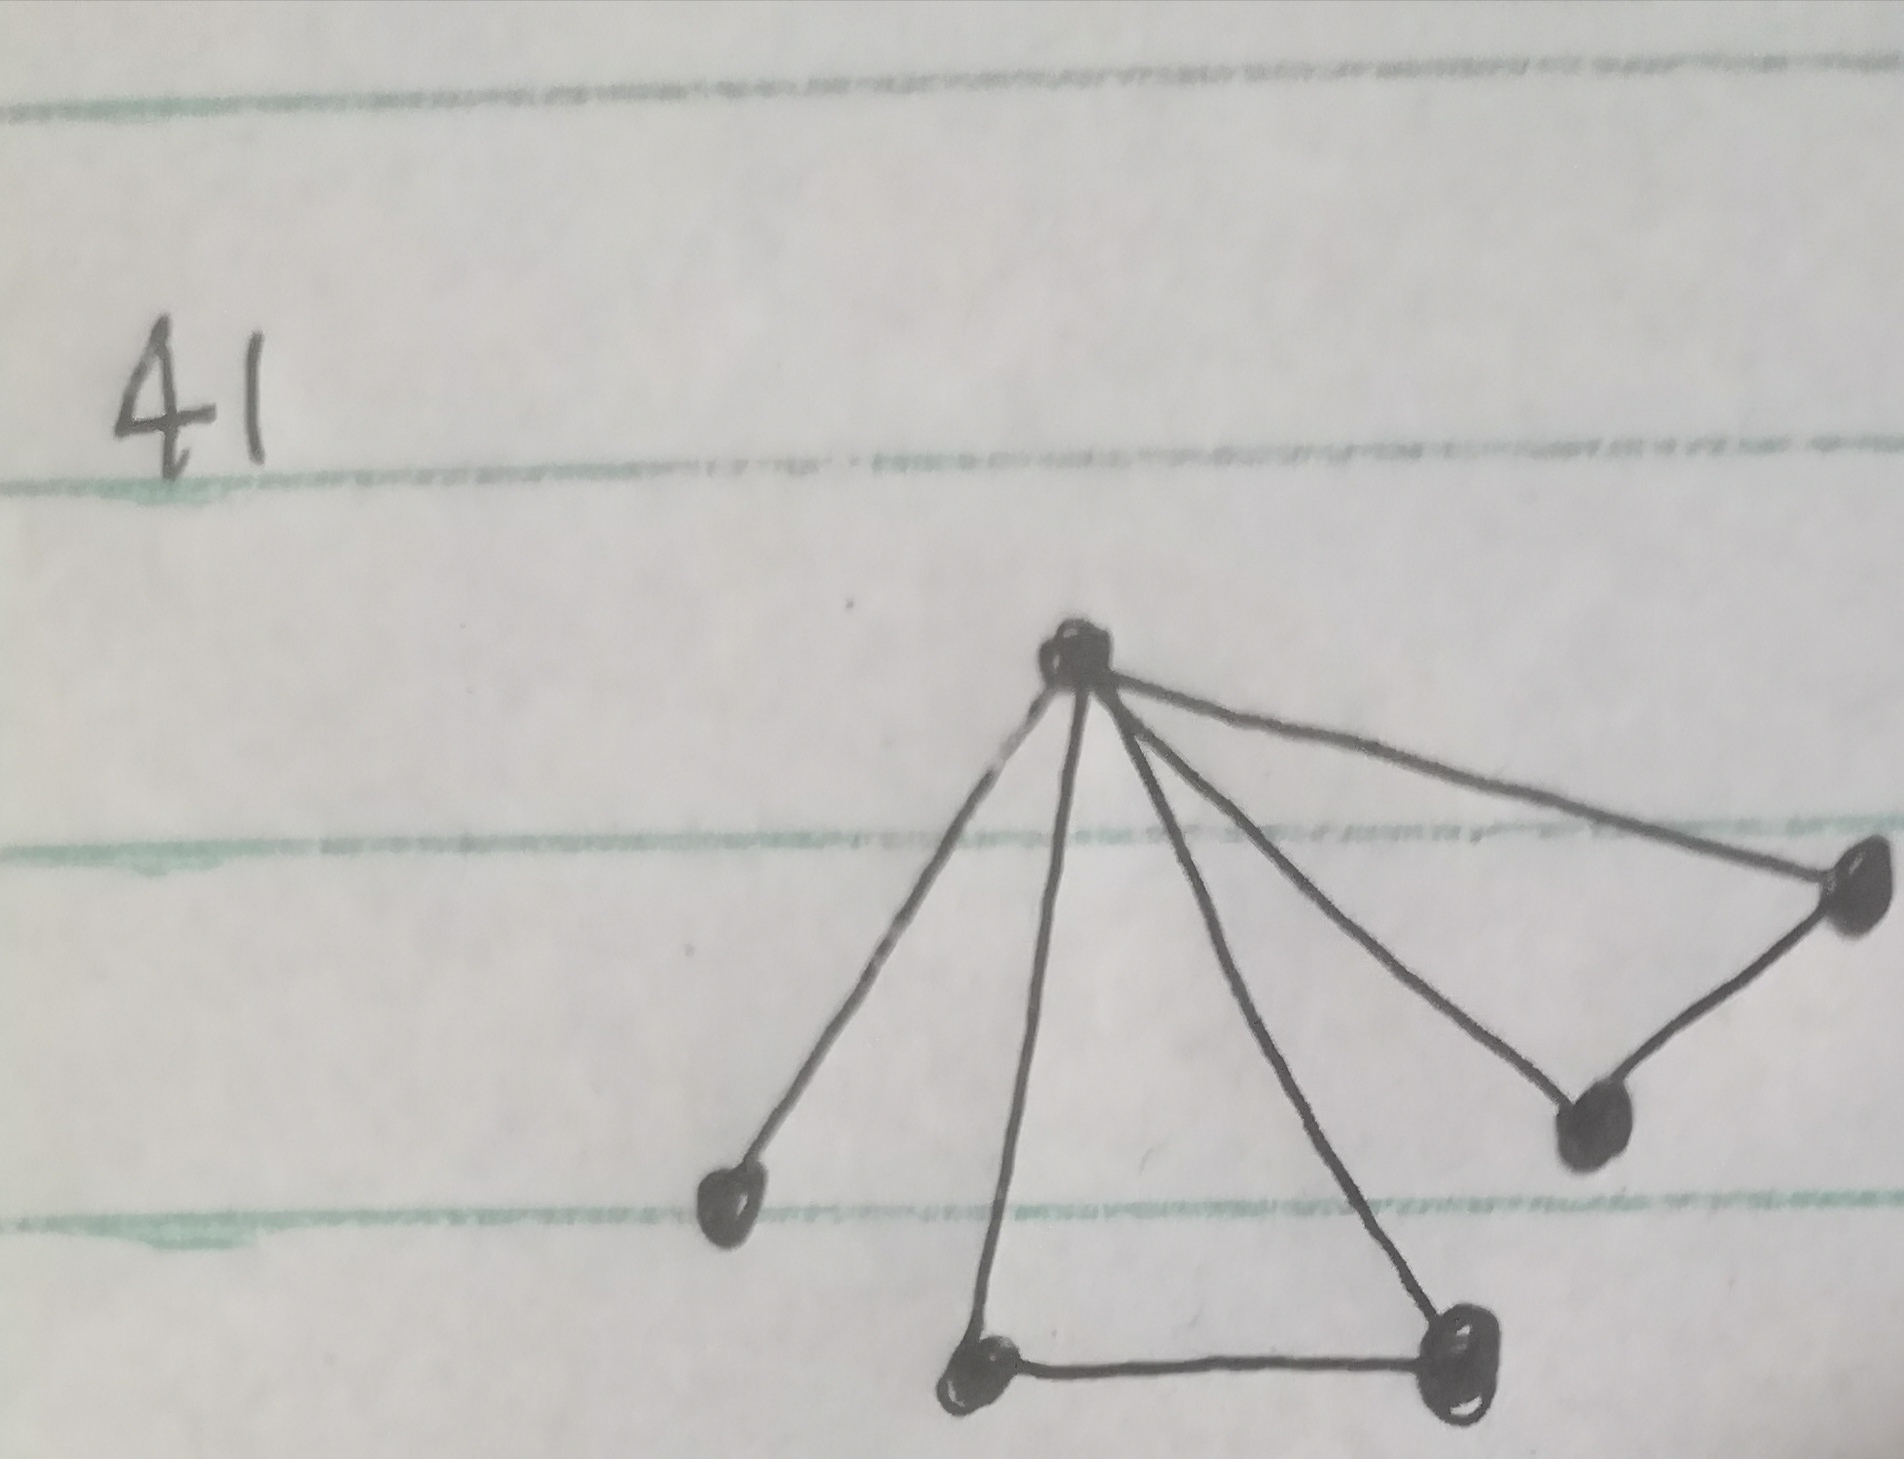
\includegraphics[scale=0.1]{../imgs/10_2_41.jpg}


    \item[53]For which values of $n$ are these graphs regular? 

            a) $K_n$                                              \\
            b) $C_n$                                              \\
            c) $W_n$                                              \\
            d) $Q_n$                                              \\

            a) $n>=1$                                              \\
            b) $n>=3$                                              \\
            c) $3$                                              \\
            d) $n>=0$                                              \\
\end{description}

\end{document}
